% 1996 上海(理) 第18题: 正三角形 ABC, E,F 为 AB,AC 中点, AD,EH,FG 垂直 BC.
% 阴影: 顶部小三角形 AEF 与两侧三角形 EBH, FGC (竖线阴影); 中间矩形 EHGF 留白.
% 采用正三角形精确坐标: B=(-a/2,0), C=(a/2,0), A=(0,h), h=sqrt(3)a/2, a=7.
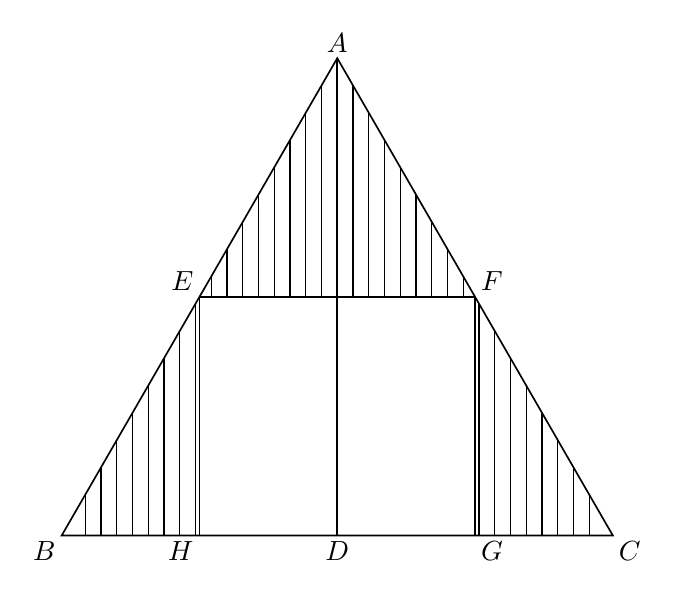
\begin{tikzpicture}[x=1cm,y=1cm,font=\normalsize,
  geo edge/.style={solid,line width=.6pt},
  geo label/.style={font=\normalsize,inner sep=2pt}]
% 顶点与垂足 (精确计算)
\coordinate (B) at (-3.50,0);
\coordinate (C) at (3.50,0);
\coordinate (A) at (0,6.06218);
\coordinate (D) at (0,0);
\coordinate (E) at (-1.75,3.03109);
\coordinate (F) at (1.75,3.03109);
\coordinate (H) at (-1.75,0);
\coordinate (G) at (1.75,0);
% 阴影区域 (竖线)



\draw[line width=.4pt] (-3.200000,0.000000)--(-3.200000,0.519615);
\draw[line width=.4pt] (-3.000000,0.000000)--(-3.000000,0.866025);
\draw[line width=.4pt] (-2.800000,0.000000)--(-2.800000,1.212436);
\draw[line width=.4pt] (-2.600000,0.000000)--(-2.600000,1.558846);
\draw[line width=.4pt] (-2.400000,0.000000)--(-2.400000,1.905256);
\draw[line width=.4pt] (-2.200000,0.000000)--(-2.200000,2.251666);
\draw[line width=.4pt] (-2.000000,0.000000)--(-2.000000,2.598076);
\draw[line width=.4pt] (-1.800000,0.000000)--(-1.800000,2.944486);
\draw[line width=.4pt] (-1.600000,3.031090)--(-1.600000,3.290897);
\draw[line width=.4pt] (-1.400000,3.031090)--(-1.400000,3.637307);
\draw[line width=.4pt] (-1.200000,3.031090)--(-1.200000,3.983717);
\draw[line width=.4pt] (-1.000000,3.031090)--(-1.000000,4.330127);
\draw[line width=.4pt] (-0.800000,3.031090)--(-0.800000,4.676537);
\draw[line width=.4pt] (-0.600000,3.031090)--(-0.600000,5.022947);
\draw[line width=.4pt] (-0.400000,3.031090)--(-0.400000,5.369358);
\draw[line width=.4pt] (-0.200000,3.031090)--(-0.200000,5.715768);
\draw[line width=.4pt] (0.000000,3.031090)--(0.000000,6.062178);
\draw[line width=.4pt] (0.200000,3.031090)--(0.200000,5.715768);
\draw[line width=.4pt] (0.400000,3.031090)--(0.400000,5.369358);
\draw[line width=.4pt] (0.600000,3.031090)--(0.600000,5.022947);
\draw[line width=.4pt] (0.800000,3.031090)--(0.800000,4.676537);
\draw[line width=.4pt] (1.000000,3.031090)--(1.000000,4.330127);
\draw[line width=.4pt] (1.200000,3.031090)--(1.200000,3.983717);
\draw[line width=.4pt] (1.400000,3.031090)--(1.400000,3.637307);
\draw[line width=.4pt] (1.600000,3.031090)--(1.600000,3.290897);
\draw[line width=.4pt] (1.800000,0.000000)--(1.800000,2.944486);
\draw[line width=.4pt] (2.000000,0.000000)--(2.000000,2.598076);
\draw[line width=.4pt] (2.200000,0.000000)--(2.200000,2.251666);
\draw[line width=.4pt] (2.400000,0.000000)--(2.400000,1.905256);
\draw[line width=.4pt] (2.600000,0.000000)--(2.600000,1.558846);
\draw[line width=.4pt] (2.800000,0.000000)--(2.800000,1.212436);
\draw[line width=.4pt] (3.000000,0.000000)--(3.000000,0.866025);
\draw[line width=.4pt] (3.200000,0.000000)--(3.200000,0.519615);
% 轮廓
\draw[geo edge] (A)--(B)--(C)--cycle;
\draw[geo edge] (E)--(F);
\draw[geo edge] (A)--(D);
\draw[geo edge] (E)--(H);
\draw[geo edge] (F)--(G);
% 标签: 完整节点, 紧邻对应点
\node[geo label,above]       at (A) {$A$};
\node[geo label,below left]  at (B) {$B$};
\node[geo label,below right] at (C) {$C$};
\node[geo label,below]       at (D) {$D$};
\node[geo label,below left]  at (H) {$H$};
\node[geo label,below right] at (G) {$G$};
\node[geo label,above left]  at (E) {$E$};
\node[geo label,above right] at (F) {$F$};
\end{tikzpicture}
